\section{Implementation}
The Music Player module consists of a number of classes, where the most notable are \texttt{DynamicQueue}, \texttt{MusicPlayerActivity}, and \texttt{MusicPlayerService}. \texttt{DynamicQueue} handles navigation, and it makes sure the queue of songs matches the user's running speed. \texttt{MusicPlayerActivity} shows a UI on the screen and handles user inputs, including navigation and volume changes. \texttt{MusicPlayerService} handles the actual playback of songs, and because it is implemented as a service, it is possible to keep playing songs in the background, i.e., without requiring \texttt{MusicPlayerActivity} to be visible.

\subsection{DynamicQueue}
\label{sec:dynamicQueue}
This class is named based on the fact that it will update dynamically, depending on the pace of the user. \texttt{DynamicQueue} utilises two queues to keep track of previously played and upcoming songs.
Each queue has a fixed size, so only the desired amount of songs will be stored at any given times, and only songs matching a given tempo are loaded into the queue for upcoming songs. 
Additionally, to prevent simply replaying the same songs over and over, all the songs in the two queues must be unique.

\subsection{MusicPlayerActivity}
This is the central point of the application, responsible for managing the rest of the application, and giving the user a way of interacting with it. It starts the \texttt{MusicPlayerService}, calls the \texttt{DynamicQueue} for songs to play, attaches listeners to the buttons, making them clickable. It also checks that there are enough songs in the specified folder, sending the user to the settings menu if this is not the case.

In order to manage the responsibilities associated with the activity, general initialisation has its own class \texttt{Initializers}. \texttt{Initializers} is responsible for setting \texttt{onClickListeners} for the GUI, and preparing the first song in the queue and coverflow. 

\subsection{MusicPlayerService} 
The \texttt{MusicPlayerServce} handles the playing of the music files. This is done with the \texttt{MediaPlayer} class, which is part of the \citet{android:MediaPlayer} API. The service is responsible for setting up event listeners, and acts as an interface to the \texttt{MediaPlayer}.  

We only used of one the two listeners available for the \texttt{MediaPlayer}, the \texttt{onCompleteListener}. This listener is called when a file reaches its end. In this event the method attached to the listener, selects the next song in Queue, by calling the \texttt{nextSong} method. 

The \texttt{onCompleteListener} is also called when an error occurs while the \texttt{MediaPlayer} is playing. In our application an illegal state error could happen if one calls \texttt{stop} while the \texttt{MediaPlayer} was not playing, triggering the \texttt{onCompleteListener}, and changing the song to the next in the queue. This was handled in the \texttt{MusicPlayerService} by ignoring \texttt{stop} or other calls, if the \texttt{MediaPlayer} was in the wrong state. 

The \texttt{MediaPlayer}'s state diagram can be seen in \cref{fig:medaiPlayerState}. The application ends up in an illegal state every time a method is called from a state, which does not have a corresponding transition. An example could be that \texttt{prepare} was called from the \texttt{started} state. One would have to call \texttt{stop} before \texttt{prepare} could be called again.

\begin{figure}[h!]
  \centering
    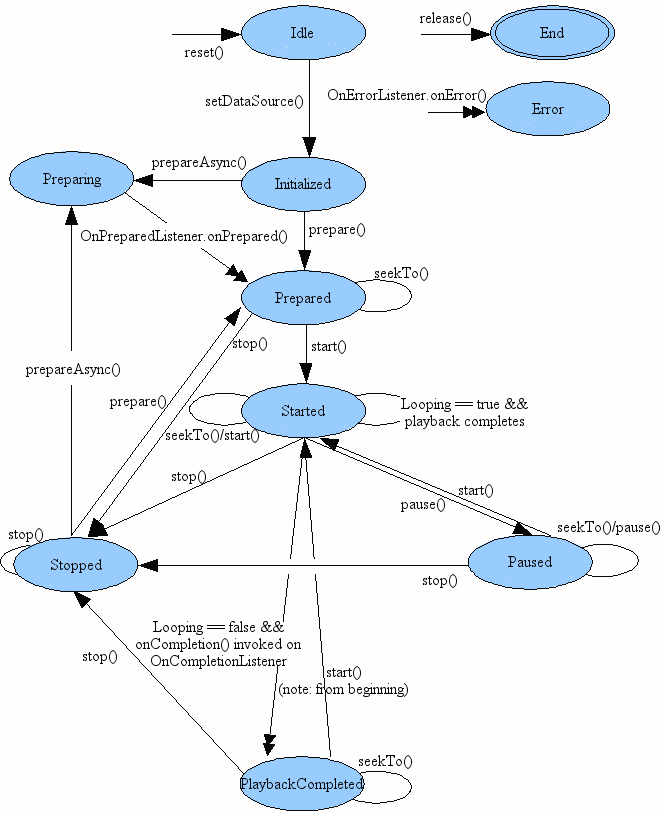
\includegraphics[width=\textwidth]{Images/mediaplayerStateDiagram.png}
  \caption{A state diagram which shows a MediaPlayer object's life cycle. Taken from \citet{android:MediaPlayer}.}
  \label{fig:medaiPlayerState}
\end{figure}
